\section{Backup}


\begin{frame}
    \frametitle{Variazioni frontali}
    \framesubtitle{}

    \begin{figure}
        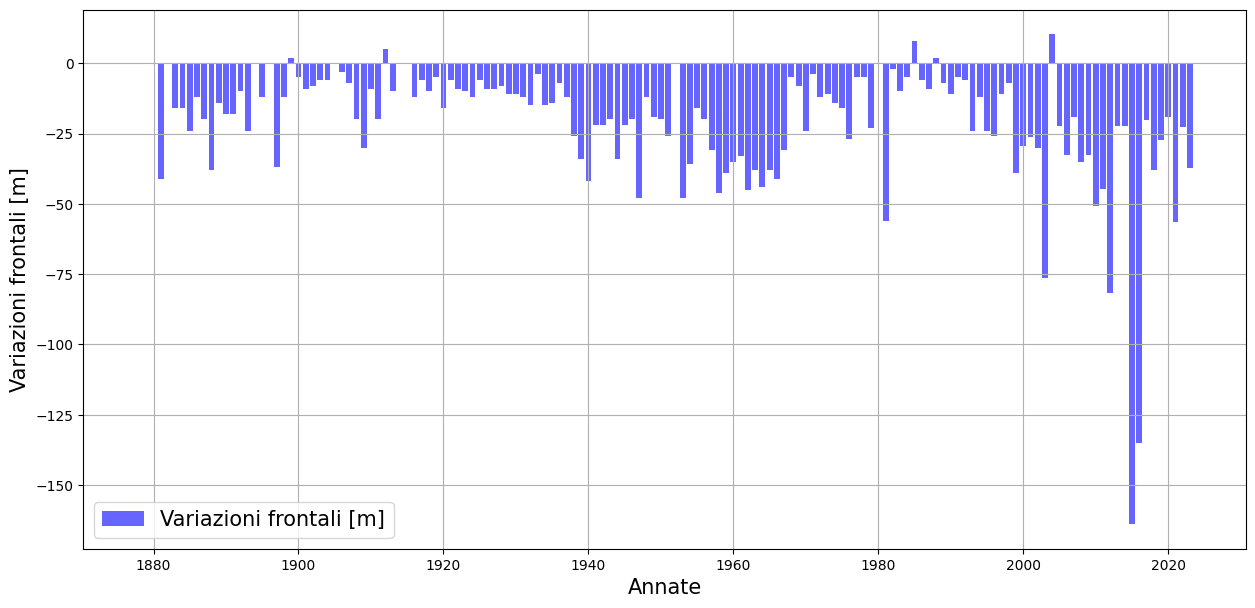
\includegraphics[width=0.9\textwidth]{Immagini/variazioniFrontali.png}
        \caption{Dati da \cite{GLAMOS23}}
    \end{figure}
  
\end{frame}


\begin{frame}
    \frametitle{Variazioni cumulate}
    \framesubtitle{}

    \begin{figure}
        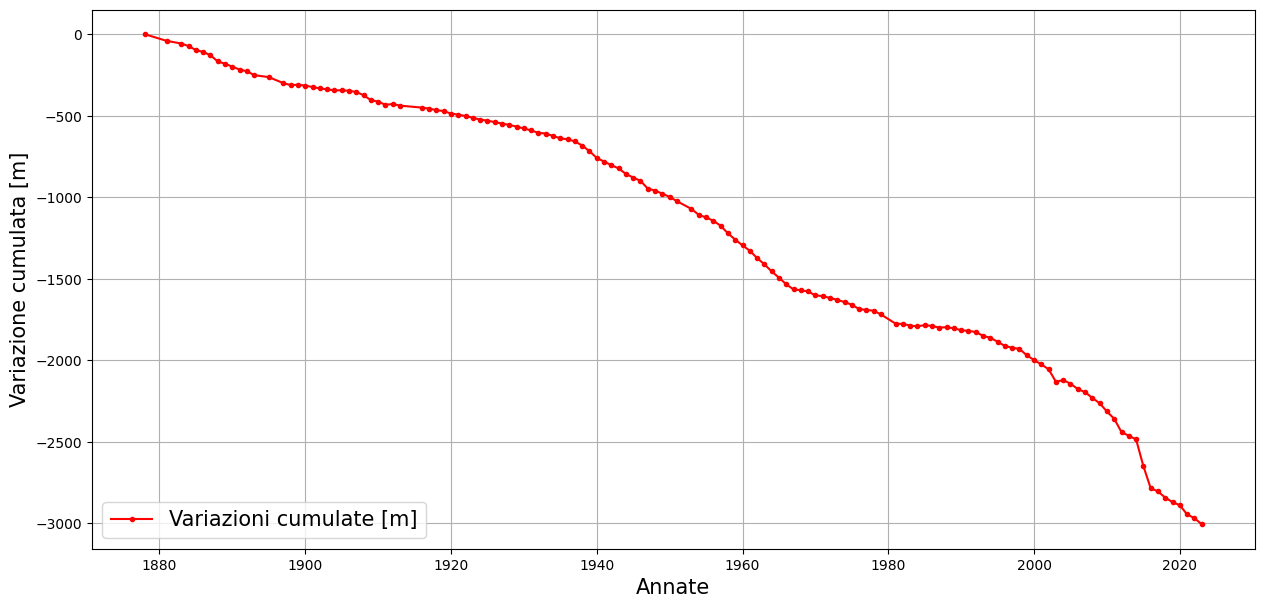
\includegraphics[width=0.9\textwidth]{Immagini/variazioniCumulative.png}
        \caption{Dati da \cite{GLAMOS23}}
    \end{figure}
  
\end{frame}


\begin{frame}
    \frametitle{Short-wave radiation}
    \framesubtitle{}

    \begin{figure}
        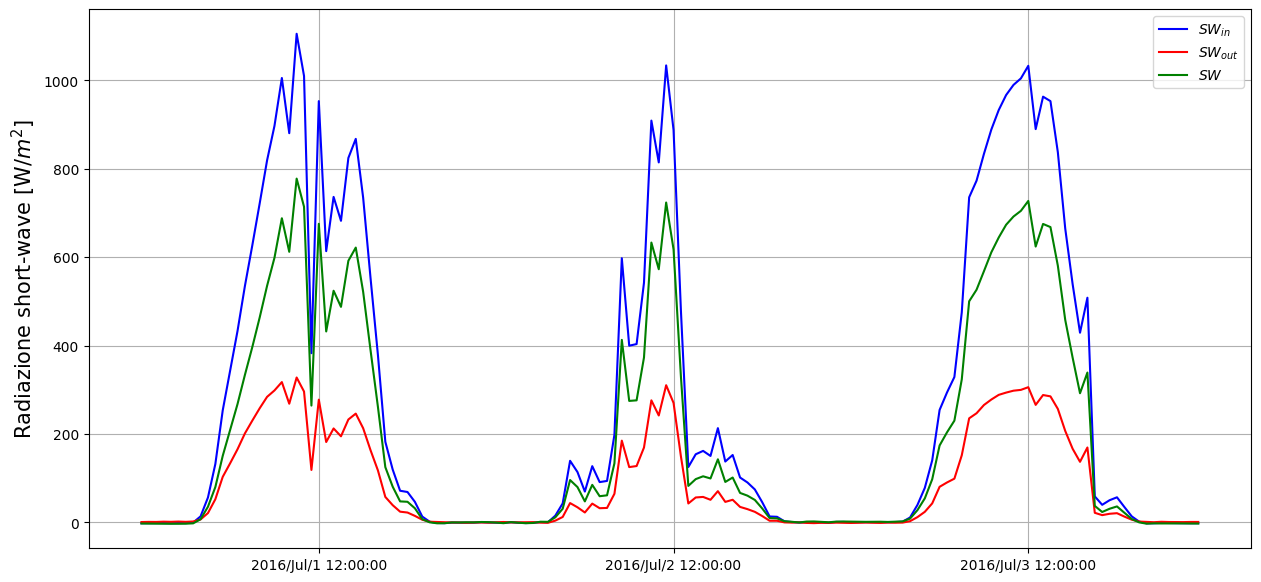
\includegraphics[width=0.9\textwidth]{Immagini/shortWave.png}
        \caption{Dati da Oerlemans}
    \end{figure}
  
\end{frame}


\begin{frame}
    \frametitle{Long-wave radiation}
    \framesubtitle{}

    \begin{figure}
        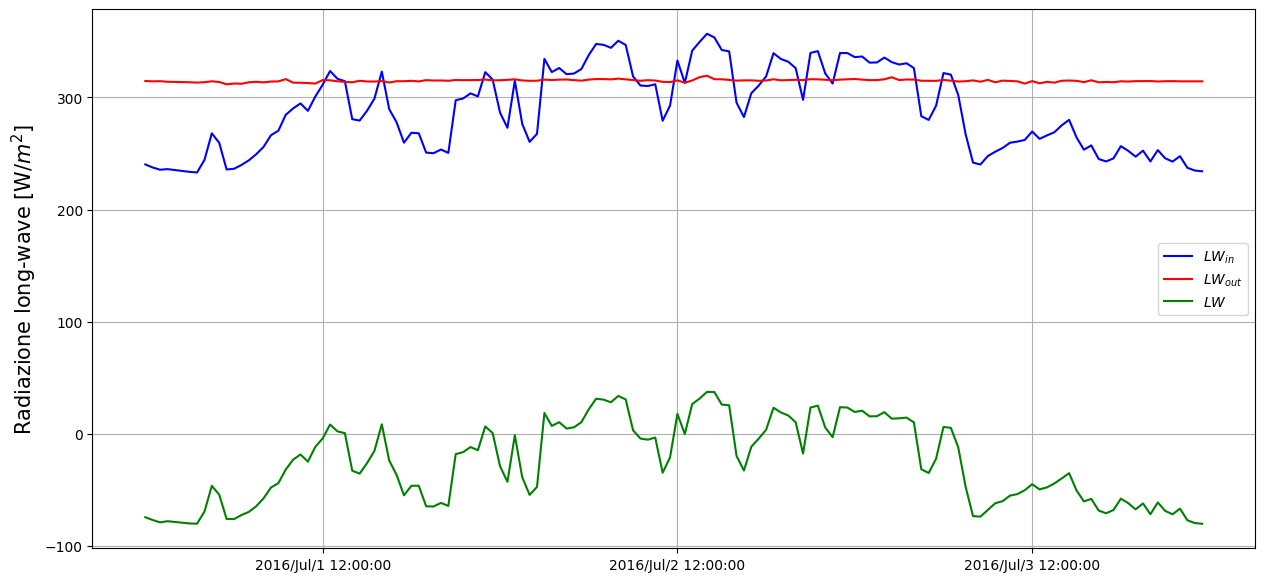
\includegraphics[width=0.9\textwidth]{Immagini/longWave.png}
        \caption{Dati da Oerlemans}
    \end{figure}
  
\end{frame}


\begin{frame}
    \frametitle{Albedo}
    \framesubtitle{}

    \begin{figure}
        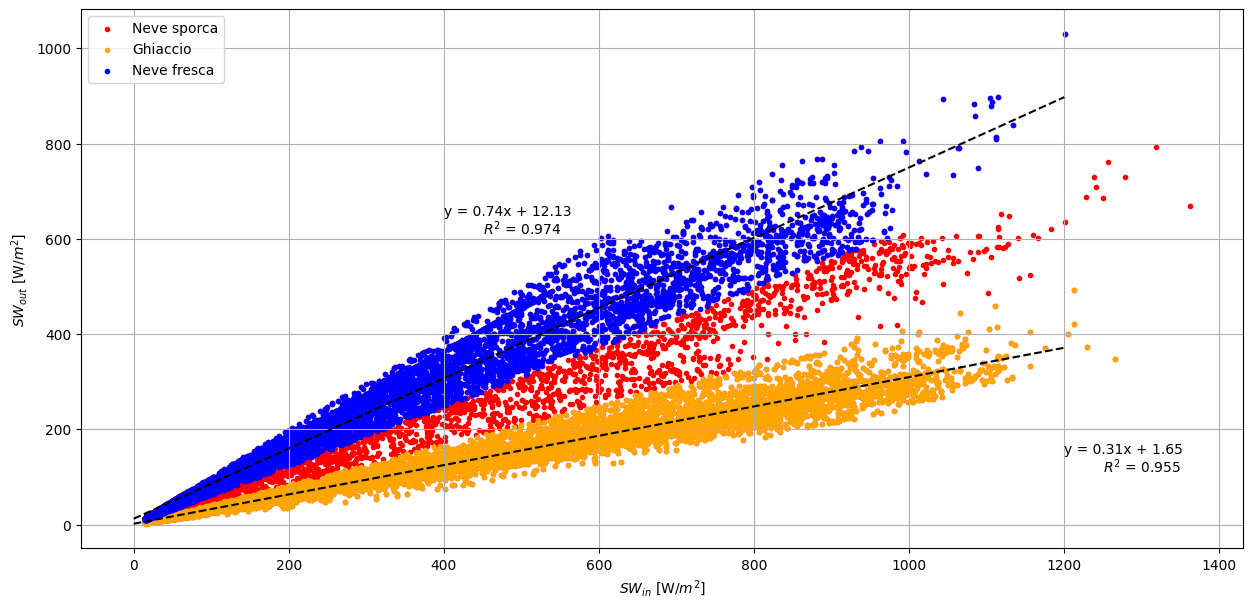
\includegraphics[width=0.9\textwidth]{Immagini/albedoHour.png}
        \caption{Dati da Oerlemans}
    \end{figure}
  
\end{frame}


\begin{frame}
    \frametitle{Temperatura}
    \framesubtitle{}

    \begin{figure}
        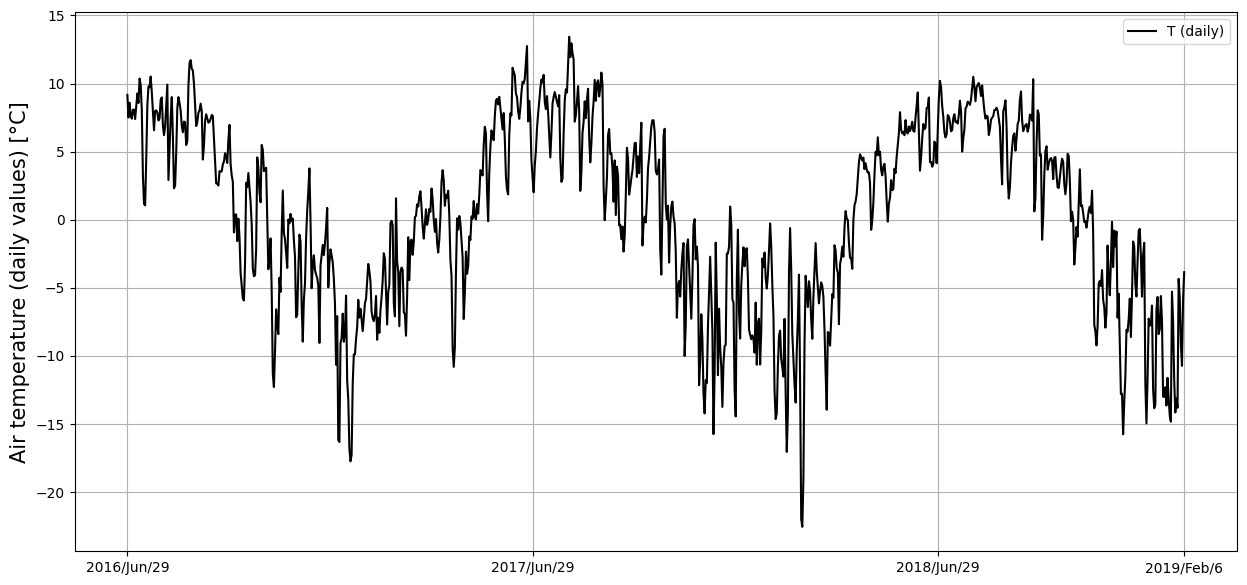
\includegraphics[width=0.9\textwidth]{Immagini/tempAria.png}
        \caption{Dati da Oerlemans}
    \end{figure}
  
\end{frame}


\begin{frame}
    \frametitle{Temperatura superficiale}
    \framesubtitle{}

    \begin{figure}
        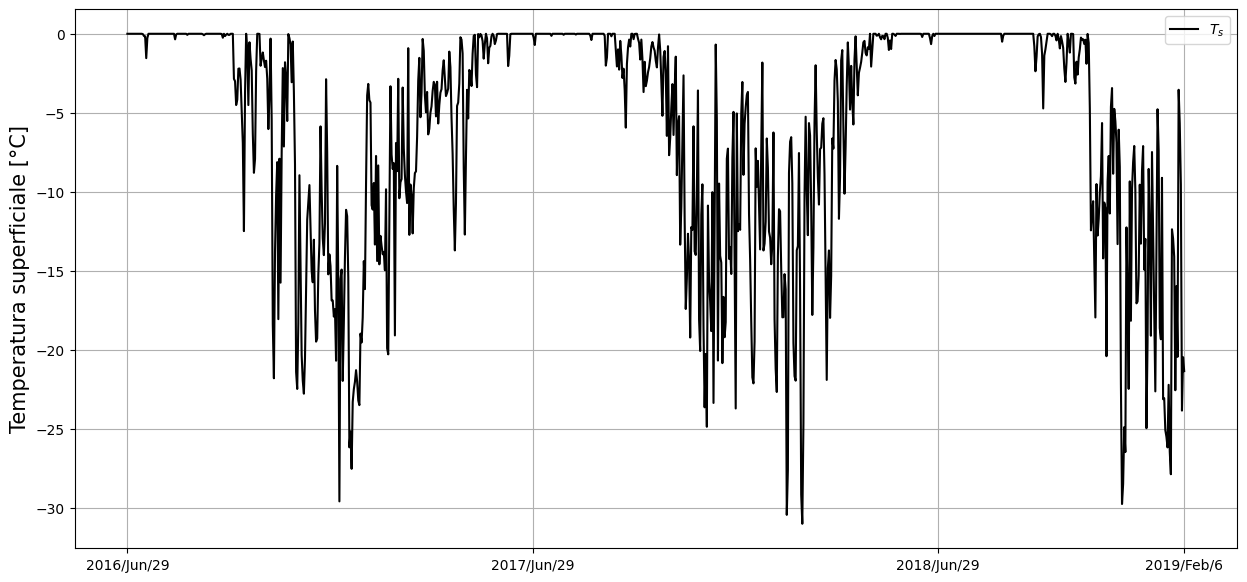
\includegraphics[width=0.9\textwidth]{Immagini/temperaturaYear.png}
        \caption{Dati da Oerlemans}
    \end{figure}
  
\end{frame}


\begin{frame}
    \frametitle{Sensible Heat e Latent Heat}
    \framesubtitle{}

    \center
    \begin{minipage}{0.5\textwidth}
        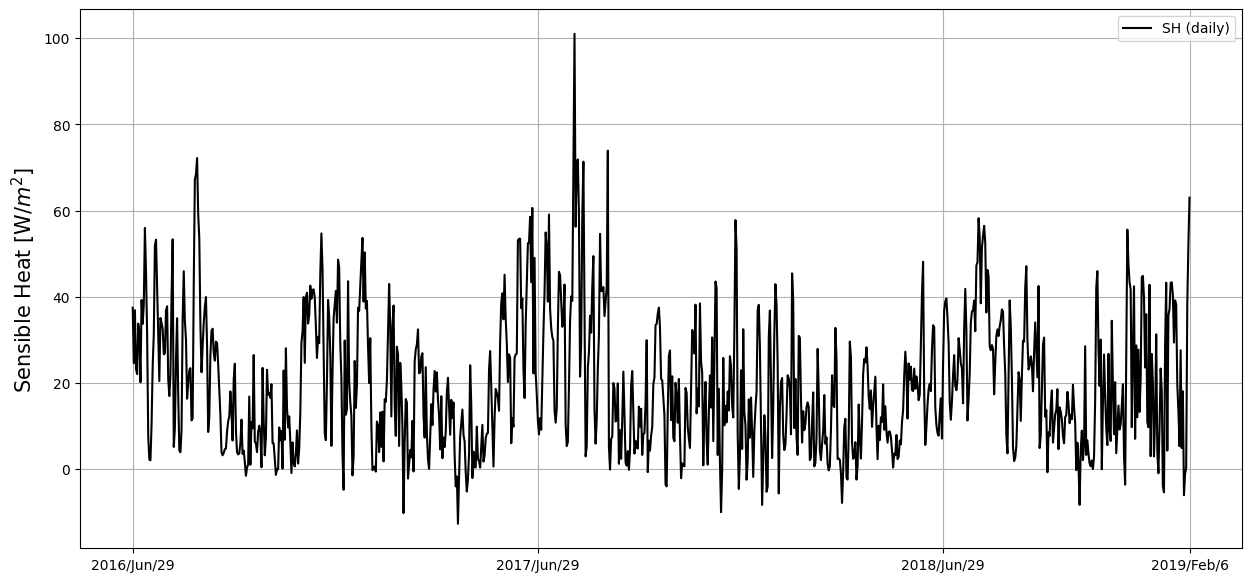
\includegraphics[width=\textwidth]{Immagini/sensibleHeatYear.png}
    \end{minipage}
    \begin{minipage}{0.5\textwidth}
        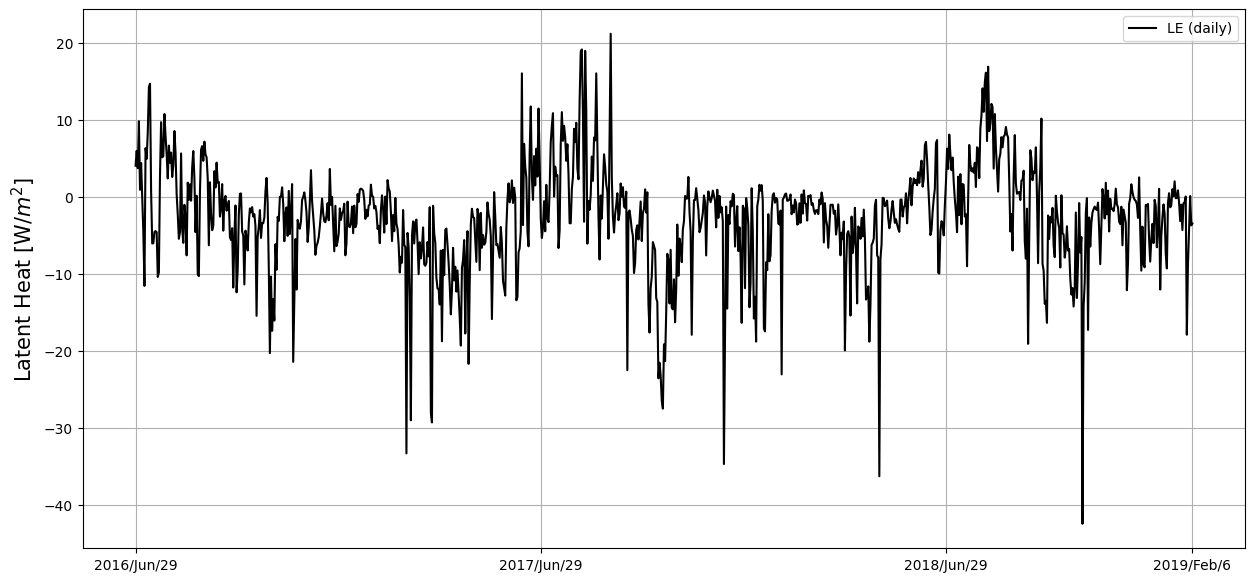
\includegraphics[width=\textwidth]{Immagini/latentHeatYear.png}
    \end{minipage}
  
\end{frame}


\begin{frame}
    \frametitle{Secondo approccio: temperatura superficiale}
    \framesubtitle{}

    \begin{figure}
        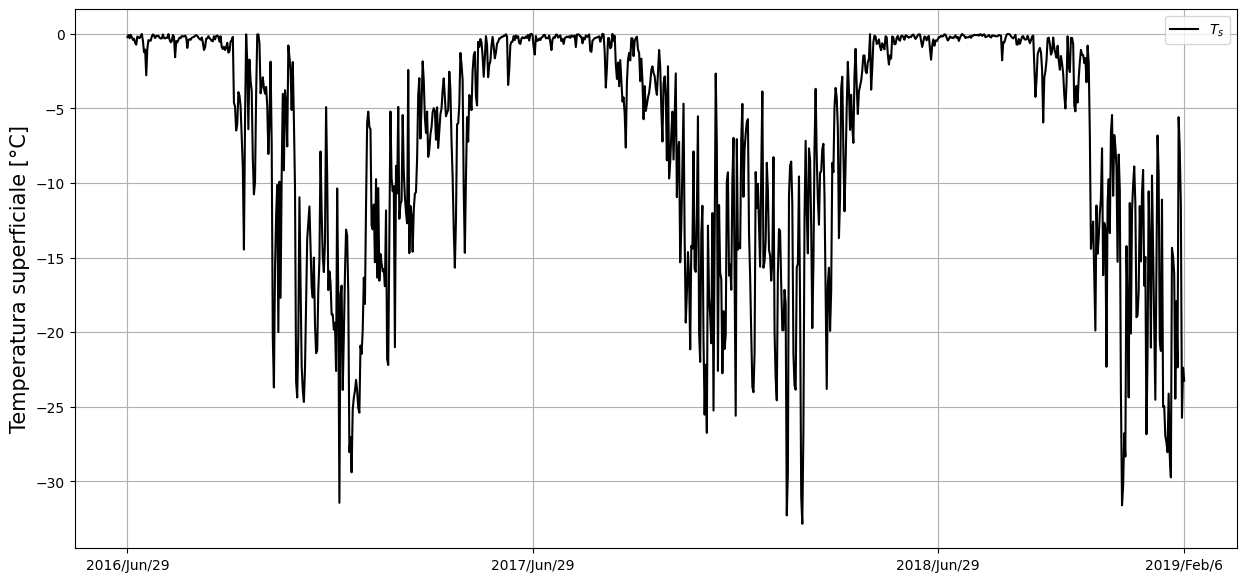
\includegraphics[width=0.9\textwidth]{Immagini/tSupAlt.png}
        \caption{Dati da Oerlemans}
    \end{figure}
  
\end{frame}


\begin{frame}
    \frametitle{Secondo approccio: sensible e latent heat flux}
    \framesubtitle{}

    \center
    \begin{minipage}{0.5\textwidth}
        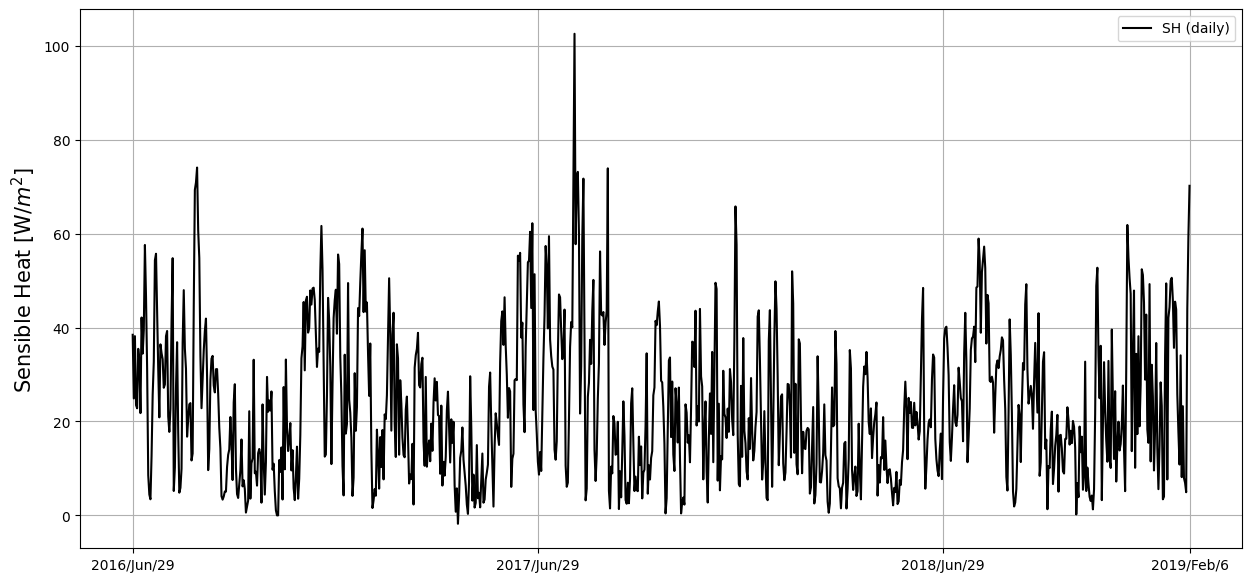
\includegraphics[width=\textwidth]{Immagini/sensibleAlt.png}
    \end{minipage}
    \begin{minipage}{0.5\textwidth}
        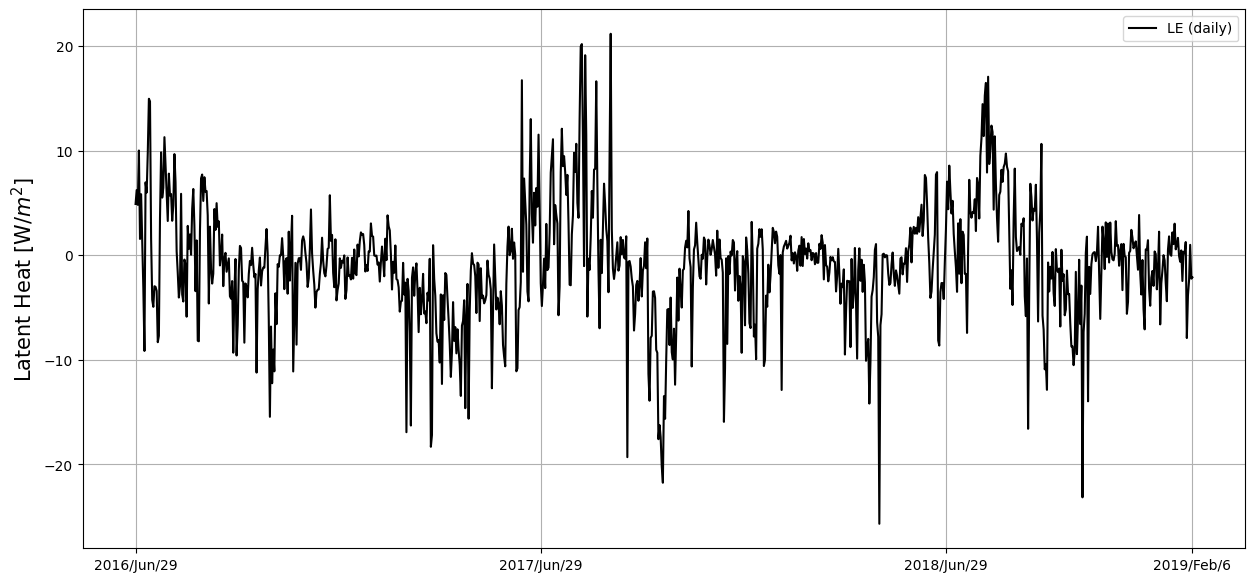
\includegraphics[width=\textwidth]{Immagini/latentAlt.png}
    \end{minipage}

\end{frame}


\begin{frame}
    \frametitle{Secondo approccio: budget energetico}
    \framesubtitle{}

    \begin{figure}
        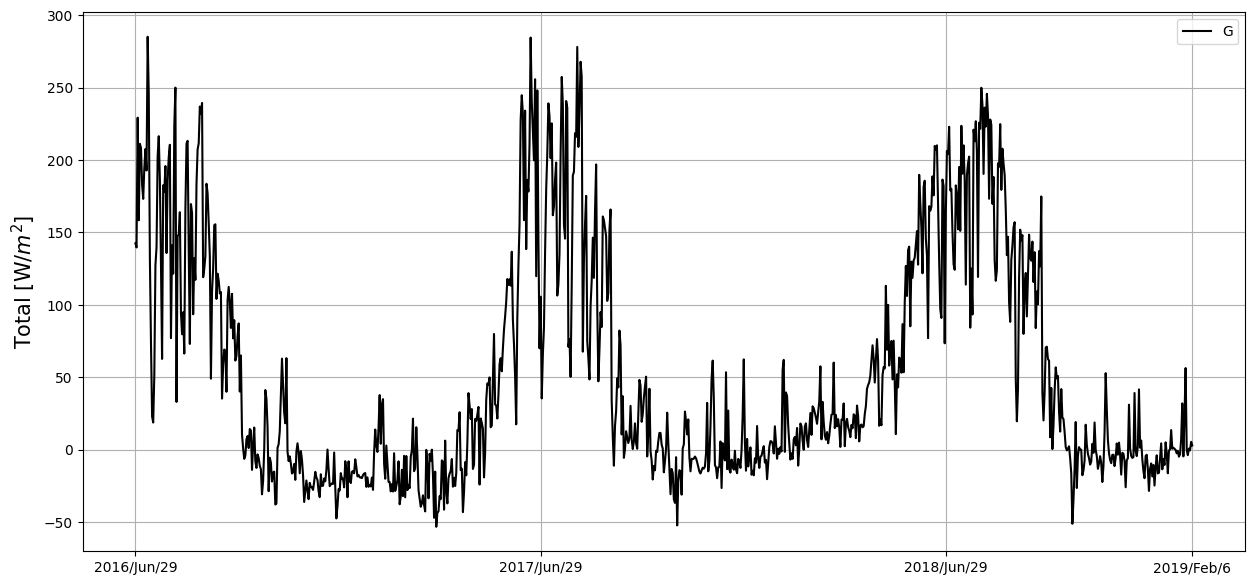
\includegraphics[width=0.9\textwidth]{Immagini/totalAlt.png}
        \caption{Dati da Oerlemans}
    \end{figure}
  
\end{frame}


\begin{frame}
    \frametitle{Secondo approccio: confronto fra modello e misurazioni}
    \framesubtitle{}

    \begin{figure}
        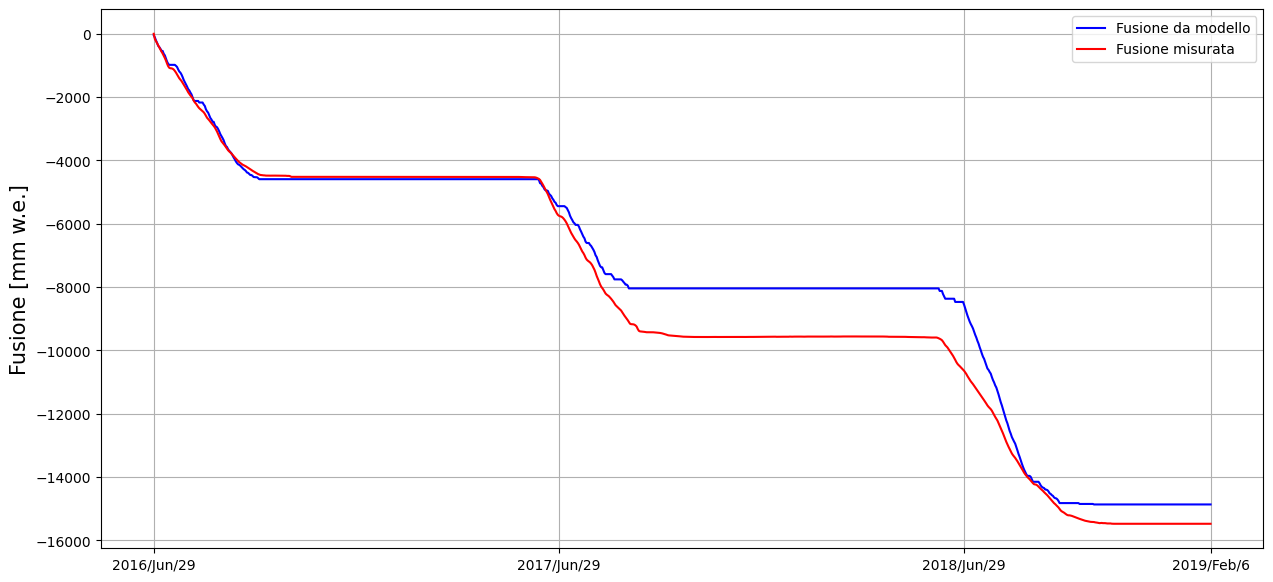
\includegraphics[width=0.9\textwidth]{Immagini/fusioneAlt.png}
        \caption{Dati da Oerlemans}
    \end{figure}
  
\end{frame}